\documentclass[14pt, fleqn, xcolor={dvipsnames, table}]{beamer}
\usepackage[T2A]{fontenc}
\usepackage[utf8]{inputenc}
\usepackage[english,russian]{babel}
\usepackage{amssymb,amsfonts,amsmath,mathtext}
\usepackage{cite,enumerate,float,indentfirst}
\usepackage{cancel}

\usepackage{tikz}                   
\usetikzlibrary{shadows}

% \usepackage{enumitem}
% \setitemize{label=\usebeamerfont*{itemize item}%
%   \usebeamercolor[fg]{itemize item}
%   \usebeamertemplate{itemize item}}

\graphicspath{{images/}}

\usetheme{Madrid}
\usecolortheme{seahorse}
\renewcommand{\CancelColor}{\color{red}}
\newenvironment{mydescription}[1]
  {\begin{list}{}%
   {\renewcommand\makelabel[1]{\color{blue}##1:\hfill}%
   \settowidth\labelwidth{\makelabel{#1}}%
   \setlength\leftmargin{\labelwidth}
   \addtolength\leftmargin{\labelsep}}}
  {\end{list}}  

\setbeamercolor{footline}{fg=Blue!50}
\setbeamertemplate{footline}{
  \leavevmode%
  \hbox{%
  \begin{beamercolorbox}[wd=.333333\paperwidth,ht=2.25ex,dp=1ex,center]{}%
    И. Кураленок, Н. Поваров, Яндекс
  \end{beamercolorbox}%
  \begin{beamercolorbox}[wd=.333333\paperwidth,ht=2.25ex,dp=1ex,center]{}%
    Санкт-Петербург, 2013
  \end{beamercolorbox}%
  \begin{beamercolorbox}[wd=.333333\paperwidth,ht=2.25ex,dp=1ex,right]{}%
  Стр. \insertframenumber{} из \inserttotalframenumber \hspace*{2ex}
  \end{beamercolorbox}}%
  \vskip0pt%
}
\newcommand\indentdisplays[1]{%
     \everydisplay{\addtolength\displayindent{#1}%
     \addtolength\displaywidth{-#1}}}
\newcommand{\itemi}{\item[\checkmark]}

\title{Машинное обучение: обзор целевых функций\\\small{}}
\author[]{\small{%
И.~Куралёнок,
Н.~Поваров}}
\date{}

\begin{document}

\begin{frame}
\maketitle
\small
\begin{center}
\vspace{-60pt}
\normalsize {\color{red}Я}ндекс \\
\vspace{80pt}
\footnotesize СПб, 2013
\end{center}
\end{frame}

\section{Введение в проблематику и классификация целевых функций}
\begin{frame}{Задача на сегодня}
\textit{Строить варианты целевой функции на заданную тему.}\\
~\\
Для этогого нам понадобится:
\begin{itemize}
  \item узнать чем отличается измерение от оптимизации;
  \item понять какие существуют подходы к построению целевой функции;
  \item научиться строить целевые функции для заданных примеров (это уже ДЗ).
\end{itemize}
\end{frame}

\begin{frame}{Пример}
Вахтер хочет понять кого пускать в парадную. Он хочет минимизировать свою работу (больше спать) по:
\begin{itemize}
   \item проверке входящих;
   \item разборкам с жильцами/руководством;
   \item уборке/проветриванию.
\end{itemize}
Для этого ему надо проверять входящих (думать).
Однако, минимизировать ``время сна'' напрямую очень сложно. Наша задача помочь бедному вахтеру.
\end{frame}

\begin{frame}{Суть проблемы}
Если мы понимаем чего хотим: $\mathcal{M}(F)(X)$ (линейка позволяющая измерить конкретное решение), то задачу оптимизации можно переписать так:
$$
\max_{\mathcal{T}} \mathcal{M} \left(\arg\max_{F} \mathcal{T}(F, L)\right)(T)
$$
Если выборка не смещена по параметрам оптимизации, то К.О. говорит нам:
$$
\mathcal{M} \equiv \arg \max_{\mathcal{T}} \mathcal{M}\left(\arg\max_{F} \mathcal{T}(F, L)\right)(T)
$$
Однако, все не так просто.
\end{frame}

\begin{frame}{Про вахтера в новых обозначениях}
\begin{mydescription}{$\mathcal{M}$}
  \item[$F$] способы проверки входящих ($F: X \to \{0,1\}$);
  \item[$\mathcal{M}$] $\mathcal{M}(X,F_0) = t_0 - \sum_{(x,y_a,y_b)} (y_a F_0(x) + y_b (1 - F_0(x))$ время сна;
  \item[$\mathcal{T}$] способы оценить проверку входящих:
\end{mydescription}
\only<2>{
  {\color{blue} Вариант 1}\\
  Преобразуем таргет:
  $$\begin{array}{ll}
  \mathcal{M}(X,F_0) &= t_0 - \sum_{(x,y_a,y_b)} (y_a F_0(x) + y_b (1 - F_0(x)) \\
  & =  t_0 - \sum_{y_b} y_b - \sum_{(x,y_a,y_b)} (y_a - y_b)F_0(x) \\
  & =  C - \sum_{(x,y_a,y_b)} (\delta y)F_0(x) \\
  \end{array}$$.
}
\only<3>{
  {\color{blue} Вариант 2}\\ \small
  Предположим, что посетителей много, и нету таких, которые доставляют особенно сильно. Тогда задача сводится к определению ``жалобщиков'':
  $$\begin{array}{ll}
  \mathcal{M}(X,F_0) &= t_0-\bar{|\delta y|} \sum_{(x, y)} sign(\delta y) (-1)^{F_0(x)} \\
  \mathcal{T}(X,p) &= \sum I\{\delta y \le 0\} \log p(x) + I\{\delta y > 0\}\log \left(1-p(x)\right) \\
  F_0 &= \left[\begin{array}{l}0, p(x) \le 0.5\\ 1, p(x) > 0.5\\ \end{array}\right.
  \end{array}$$
  В этом случае, можно рассматривать $y'$ как новую цель, и решать задачу классификации в $T = p(X|F)$, где $p$ --- вероятность проблемности
}
\only<4>{
  {\color{blue} Вариант 3}\\
  На практике делать опрос типа: ``а вы бы жаловаться пошли?'' --- не удобно, поэтому можно иначе:
  $$\begin{array}{c}
  \mathcal{T}(X_a, F') = \sum_{(x,y_a)} \left(y_a - F'(x)\right)^2\\
  \mathcal{T}(X_b, F'') = \sum_{(x,y_b)} \left(y_b - F''(x)\right)^2\\
  F(x) = \left\{\begin{array}{ll}
  0 & F'(x) > F''(x)\\
  1 & F'(x) \le F''(x) \\
  \end{array}\right.
  \end{array}$$.
}

\end{frame}

\begin{frame}{Проблема в построении}
Что может быть ``не так'' в очевидном решении:
\begin{itemize}
  \item $\mathcal{M}$ может быть неудобна для оптимизации (кусочно-постоянная, например);
  \item сложно гарантировать несмещенность по параметрам оптимизации;
  \item сложно собирать данные в терминах $\mathcal{M}$;
\end{itemize} 
Поэтому все еще актуально решать исходную задачу:
$$
\max_{\mathcal{T}} \mathcal{M} \left(\arg\max_{F} \mathcal{T}(F, L)\right)(T)
$$
\end{frame}

\begin{frame}{Как можно подойти к построению $\mathcal{T}$}
Можно исходить из трех соображений:
\begin{enumerate}
  \item {\color{blue}$\mathcal{T} \equiv \mathcal{M}$:} усреднение $\mathcal{M}$ по всему доступному опыту;
  \item {\color{blue}$\max_{\mathcal{T}} \mathcal{M} \left(\arg\max_{F} \mathcal{T}(F, L)\right)(T)$:} вероятностное моделирование происходящего: как можно получить $\mathcal{M}$ из удобного $\mathcal{T}$.
  \item {\color{blue}$\arg\max_{F} \mathcal{T}(F, L) = \arg\max_{F} \mathcal{M}(F, L)$:}~\\
  \begin{itemize}
    \item регрессия по ``очкам'': введем для каждого наблюдения стоимость, и будем ее приближать по $\mathcal{T}$;
    \item принцип максимальной энтропии;
    \item принцип минимального описания;
  \end{itemize}
\end{enumerate} 
\end{frame}

\section{Способы усреднения}

\begin{frame}{Средние значения}
Будем оценивать каждое наблюдение. Хотим улучшить результат в среднем.
$$
F_0 = \arg \max_F \frac{1}{n} \sum_i \mathfrak{m}(F(x_i),y_i)
$$
Поделили большую $\mathcal{M}$ на много маленьких $\mathfrak{m}$. 
\begin{description}
\small
\leftmargin=-5em
\itemindent=0em
\labelwidth=0em
\leftskip=-5em
  \item[\color{green}+] по наблюдениям делить естественно;
  \item[\color{red}---] надо следить за независимостью наблюдений;
  \item[\color{red}---] работает только для ситуаций когда нет $\infty$ потерь/приобретений;
\end{description} 
\end{frame}

\begin{frame}{Средние значения бывают разные}
Последнюю проблему можно решить с помощью других средних:

\begin{description}
  \item[геометрическое]: $\sqrt[n]{\prod_i x_i}$; 
  \item[гармоническое]: $n\over \sum_i \frac{1}{x_i}$;
\end{description}
\end{frame}

\begin{frame}{Разные только пространства усреднения}
$$
A(\{x_i\}) = f^{-1}\left(\frac{1}{n} \sum_i f(x_i)\right)
$$
В этих терминах все средние отличаются лишь отображением $f$;
\begin{description}
  \item[арифметическое]: $f(x) = x$; 
  \item[геометрическое]: $f(x) = \log x$; 
  \item[гармоническое]: $f(x) = \frac{1}{x}$; 
\end{description}
C точки зрения оптимизации, если функция $f$ монотонная, то мы все можем отбросить и оптимизировать только
$$
\max \sum_i f(x_i)
$$
\end{frame}

\section{Очки и их учет}

\begin{frame}{Почему это работает}
Пусть задана метрика $\mathcal{M}$, хотим получить решение $F$, которое ее максимизирует. Введем дополнительную интерпретацию наблюдений $s(y_i) \in \mathbb{R}$. Будем предсказывать $s(y_i)$:
$$
F_0 = \arg\min_F \sum_i \|F(x) - s(y_i)\|_{l_q})
$$
\begin{itemize}
  \item формирование $s(y)$ --- отдельная проблема;
  \item регрессия известная задача;
  \item все гладко\footnote{для некоторых $q$ :)}, выпукло и удобно для оптимизации.
\end{itemize}
\end{frame}

\begin{frame}{Виды невязки $l_q$}
Невязку можно интерпретировать по-разному и в зависимости от интерпретации подбирать $q$:
$$
l_q(x,b) = \|x - b\|_{l_q} = \left(\sum_i\|x_i - b_i\|^q\right)^\frac{1}{q}
$$
Все чуть менее гладко, чем хотелось бы, но и такие штуки оптимизируются с помощью односторонних градиентов.
\end{frame}

\begin{frame}{Экстремальные случаи $q$}
Особенно интересны экстремальные случаи $q$:
$$\begin{array}{l}
l_0(x,b) = \sum_i I\{x = b\} \\
l_{\infty}(x,b) = max |x - b| \\
\end{array}$$
Очень понятный физический смысл, но с гладкостью беда: оптимизация $l_0$ $NP$-hard.
\end{frame}

\begin{frame}{Как выглядят разные $q$}
\centering
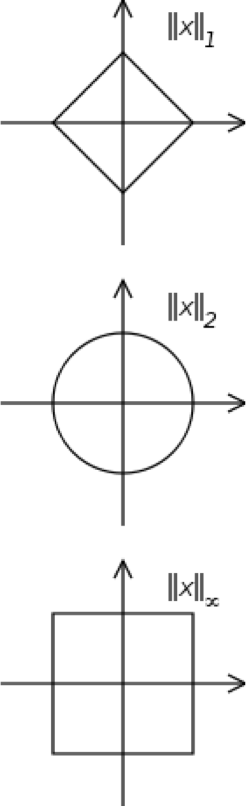
\includegraphics[width=0.2\textwidth]{lq1.png}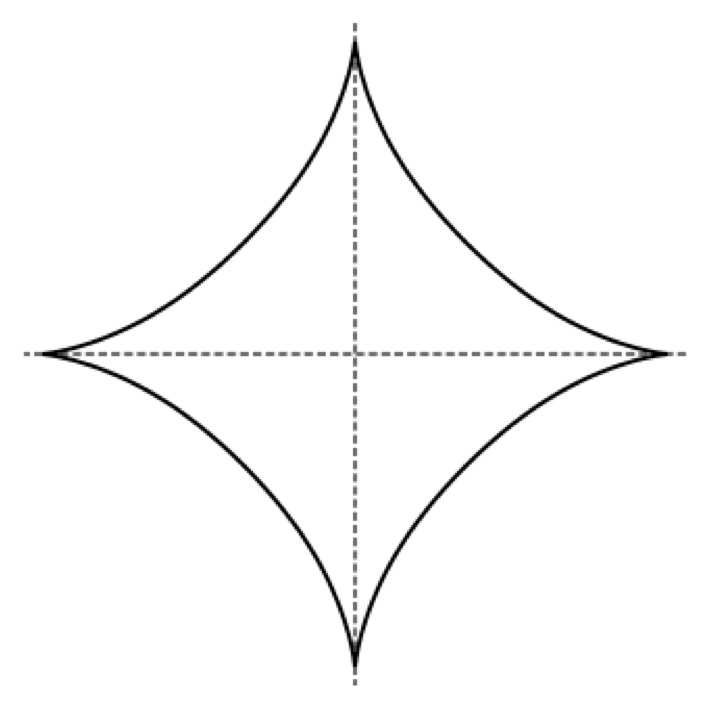
\includegraphics[width=0.65\textwidth]{lq2.png}
%Часто из $l_0$ делают $l_1$
\end{frame}

\begin{frame}{Подбираем ``очки''} % повтор
$$
\max_{s} \mathcal{M} \left(\arg\max_{F} \|F(x) - s(y)\|_{l_q}\right)(T)
$$
Обычно первая версия ``от балды''. Развиваем итеративно :).
\end{frame}

\begin{frame}{Вспоминая вахтера}
Назначим очки:

\begin{tabular}{p{0.6\textwidth}|l}
Результат & Очки \\
\hline \\
Ничего & 0 \\
Громко тусовался & 10 \\
Накурил & 15 \\
Напачкал & 100 \\
\end{tabular}

Это сильно проще сделать ``от балды'', чем считать статистику.
\end{frame}

\subsection{Вероятностные модели}

\begin{frame}{Моделирование вахтера}
Попробуем объяснить происходящее, зная как оно бывает:
\begin{description}
  \item[Местные] проблемные только если выпьют;
  \item[Не местные] бывают:
  \begin{description}
    \item[Приличные] не будут ничего плохого делать, пока не выпьют;
    \item[Неприличные] могут нахамить, могут создать проблемы.
  \end{description}
\end{description}
Составим из этой картины мира вероятностную модель, и оптимизируем ее.
\end{frame}

\begin{frame}{Оптимизация вероятностной модели}
$$
\arg \max_F p(F|X)
$$
\begin{itemize}
  \item В вероятностях проще рассуждать о жизни
  \item Интересно найти параметры, которые наиболее вероятны при наблюдаемых данных
  \item Обычно непонятно как это распределение построить напрямую
\end{itemize}
\end{frame}

\begin{frame}{Почему это работает}
Мы строим $p$ таким образом, что она отражает наше понимание о структуре области. По сути мы итеративно напрямую оптимизируем
$$
\max_{\mathcal{T}} \mathcal{M} \left(\arg\max_{F} \mathcal{T}(F, L)\right)(T)
$$
с использованием натурального интеллекта :).
\end{frame}
\begin{frame}{Байесовские методы}
$$
p(f | X) = \frac{p(X|f) p(f)}{p(X)} \sim p(X|f) p(f)
$$
Да, внизу интеграл, мы надеемся, что его можно взять и он не 0
\begin{description}
  \item[p(X|f)] правдоподобие
  \item[p(f)] априорное знание о семействе
\end{description}
$$
F(x) = \int_f p(x|f) p(f|X) df
$$
\end{frame}

\begin{frame}{Байесовские методы (практика)}
\begin{enumerate}
  \item Задаем априорное распределение параметров (например N(0,1))
  \item Вычисляем вероятность X, считая что точки независимы и одинаково распределены
  $$
  p(X|f) = \prod_i p(x_i|f)
  $$
  \item Получаем распределение из которого можно посамплить
  \item Усредняем посампленное
\end{enumerate}
\end{frame}

\begin{frame}{Байесовские методы (свойства)}
% \textbf{\color{green}Pros}
\begin{description}
  \item[\color{green}+] Все честно с точностью до входных данных и построенной модели
  \item[\color{green}+] Можно использовать информацию о предыдущем обучении (задавая prior)
  \item[\color{green}+] Можно понять погрешность предсказания (даже если она не выводится аналитически)
\end{description}
% \textbf{\color{green}Cons}
\begin{description}
  \item[\color{red}---] Все сильно зависит от выбора prior
  \item[\color{red}---] Сложная решающая функция
  \item[\color{red}---] Необходимо эффективное сэмплирование пространства решений
\end{description}
\end{frame}

\begin{frame}{Максимум апостериори}{Байес по простому}
\begin{itemize}
  \item Хочется попроще
  \item Для оценки ошибок есть бутстраппинг
  \item Ансамбли можно сделать другими способами и включить в решающую функцию
\end{itemize}

Чтобы не возиться со сложной $F$, можно просто взять самое вероятное решение:
$$
F(x) = f(x) : p(f|X) > p(g|X), \forall g \in F
$$
получим \textbf{maximum a posteriori}.
\end{frame}

\begin{frame}{Метод максимального правдоподобия}{(Байес совсем по простому)}
\begin{itemize}
  \item Лень придумывать prior
  \item Нет информации о предыдущих экспериментах
  \item Быстро меняющиеся условия
\end{itemize}
А можно совсем обнаглеть и убрать еще prior, сказав, что все решения одинаково вероятны:
$$\begin{array}{rl}
p(f) = & p(g) \forall f,g \\
\\
F = & \arg \max_F p(X|f) = \arg \max_F \prod_i p(x_i | f) \\
= & \arg \max_F \sum_i log(p(x_i | f)) = \arg \max_F LL(X, f)
\end{array}$$
Заметим, что prior не корректен, в случае $|F| = \infty$.
\end{frame}

\begin{frame}{Веса при LL}
$$\begin{array}{rl}
F = & \arg \max_F \prod_i \left(p(x_i | F)\right)^{n(\frac{w_i}{Z}N)} \\
= & \arg \max_F \prod_i \left(p(x_i | F)\right)^{w_i} \\
= & \arg \max_F \sum_i w_i \log p(x_i|F)
\end{array}$$
\begin{itemize}
  \item Важность точек может быть разной
  \item Введем «вес» для каждой точки
  \item Будем выбирать точки случайно, с вероятностью пропорциональной весу
\end{itemize}
\end{frame}

\subsection{Математические свойства ММП}

\begin{frame}{Сходимость ММП}
\begin{itemize}
  \item Идентификация (все функции разные);
  \item Множество функций компактно;
  \item Функции непрерывны с вероятностью 1;
  \item Существует мажорирующая интегрируемая $D$:
\end{itemize}
  $$
  | ln F(x) | < D(x)
  $$
  $\Longrightarrow$ при увеличении количества точек $L$ сходится
  $$
    sup\|LL(x, F) - LL(x, F_0)\| \overset{a.s.}{\to} 0
  $$
\end{frame}

\begin{frame}{Асимптотическая нормальность ММП}
\begin{itemize}
  \item Первые две производные $L$ определены:
  $$\begin{array}{l}
    F = F(x, \lambda) \\
    i_{j,k} = \mu_X(\frac{\partial^2L}{\partial\lambda_j\partial\lambda_k})
  \end{array}$$
  \item Матрица $I$ не ноль, непрерывная функция лямбды;
  \item Выполняется консистентность;
  \item И всё остальное хорошо:
  $$
  \sqrt{n}(\lambda_{mle} - \lambda_0) \overset{d}{\to} \mathcal{N}(0, I^{-1})
  $$
\end{itemize}
\end{frame}
\section{Принцип максимальной энтропии}

\begin{frame}{Принцип максимальной энтропии I}
\begin{itemize}
  \item Много Больцмана;
  \item Кажется, что энтропия может сама только увеличиваться;
  \item Если оставить систему в покое, то может быть она прийдёт к максимуму энтропии;
  \item Будем считать, что система живёт уже давно;
  \item Найдём такие параметры системы, которые обеспечивают максимальную энтропию, сохраняя априорно заданные параметры.
\end{itemize}
\end{frame}


\begin{frame}{Принцип максимальной энтропии II}
\begin{itemize}
  \item Выразим априорные свойства в виде ограничений;
  \item Найдём распределение обладающее максимальной энтропией;
  \item Когда хочется своего $p(x|I)$ решение будет другое.
\end{itemize}
$$\begin{array}{l}
\sum_i p(x_i|I)f_k(x_i) = f_k^0, k = 1, \ldots, m \\
\\
p(x|I) = \frac{1}{Z}e^{\sum_k\lambda_kf_k(x)} \\
\\
Z = \sum_i\exp^{\sum_k\lambda_kf_k(x)} \\
\\
f_k^0 = \frac{\partial}{\partial\lambda_k}logZ
\end{array}$$
\end{frame}

\begin{frame}{Почему это работает} % переход в общие термины
$\arg\max_{F} \mathcal{T}(F, L) = \arg\max_{F} \mathcal{M}(F, L)$

Максимизацией энтропии мы выпиливаем информацию про выборку, оставляя лишь информацию о генеральной совокупности. Так как мы хорошо смоделировали, надеемся, что минимум по метрике и по энтропии в одной точке.
\end{frame}

\section{Принцип наименьшего описания}

\begin{frame}{Принцип наименьшего описания}
\begin{itemize}
  \item Формализация бритвы Оккама;
  \item Колмогоров/Solomonoff;
  \item Вводим сложность по Колмогорову;
  \item Находим оптимальное решение; 
  \item По хорошему вероятность = 1.
\end{itemize}
$$
  F_0 = \arg\min_{F:p(X|F)\ge\epsilon} C(F)
$$

\end{frame}

\begin{frame}{Почему это работает} % переход в общие термины
Те же рассуждения, что и при ПМЭ.
\end{frame}

\begin{frame}{Сглаживание таргета}
\centering
Когда целевая функция "плохая":
$$
F_0 = \arg\max_F UT(X|F) = \arg\max_F \mu_{x \sim p(F)}(UT(x))
$$
\end{frame}

\begin{frame}{Чему следовать выбирая таргет}
\begin{itemize}
  \item Чувство прекрасного;
  \item Возможность применять математику:
  \begin{itemize}
    \item Скорость вычисления;
    \item Дифференцируемость (градиентные методы).
  \end{itemize}
  \item Наличие интересных внутренних параметров;
  \item Возможность проверить осмысленность промежуточных результатов.
\end{itemize}
NB: Чем больше мы в области, тем больше знания мы перенесем в таргет.
\end{frame}

\section{ДЗ}
\begin{frame}{Задание на дом}
\begin{itemize}
  \item Придумать таргеты для некоторых задач; 
  \item Точные задачи приведены в файле howto.txt; 
  \item Дедлайн 18 октября.
\end{itemize}
М.: Издательство МЦНМО, 2010
\end{frame}
\end{document}
